\documentclass[tikz,border=9pt]{standalone}
\usepackage{amsmath}
\usetikzlibrary{arrows.meta,fit}
\begin{document}
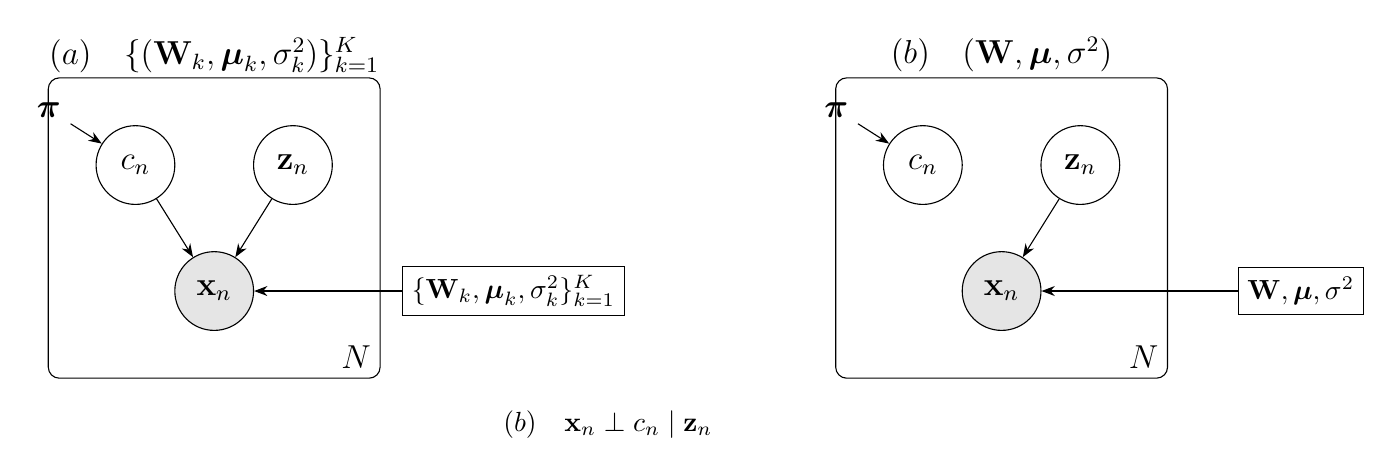
\begin{tikzpicture}[>=Stealth,latent/.style={circle,draw,minimum size=10mm},obs/.style={latent,fill=gray!20},font=\large]
\node at (0,3) {$(a)\quad\{(\mathbf W_k,\boldsymbol\mu_k,\sigma_k^2)\}_{k=1}^K$};
\node[latent] (c) at (-1,1.6) {$c_n$};
\node[latent] (z) at (1,1.6) {$\mathbf z_n$};
\node[obs] (x) at (0,0) {$\mathbf x_n$};
\draw[->] (c)--(x);\draw[->] (z)--(x);
\node (pi) at (-2.1,2.3) {$\boldsymbol\pi$};\draw[->] (pi)--(c);
\node[draw,rectangle,font=\normalsize,align=center] (theta) at (3.8,0) {$\{\mathbf W_k,\boldsymbol\mu_k,\sigma_k^2\}_{k=1}^K$};\draw[->] (theta)--(x);
\node[draw,rounded corners,fit=(c)(z)(x),inner sep=6mm] (p) {};
\node[anchor=south east] at (p.south east) {$N$};
\begin{scope}[xshift=10cm]
\node at (0,3) {$(b)\quad(\mathbf W,\boldsymbol\mu,\sigma^2)$};
\node[latent] (c2) at (-1,1.6) {$c_n$};
\node[latent] (z2) at (1,1.6) {$\mathbf z_n$};
\node[obs] (x2) at (0,0) {$\mathbf x_n$};
\draw[->] (z2)--(x2);
\node (pi2) at (-2.1,2.3) {$\boldsymbol\pi$};\draw[->] (pi2)--(c2);
\node[draw,rectangle,font=\normalsize] (theta2) at (3.8,0) {$\mathbf W,\boldsymbol\mu,\sigma^2$};\draw[->] (theta2)--(x2);
\node[draw,rounded corners,fit=(c2)(z2)(x2),inner sep=6mm] (p2) {};
\node[anchor=south east] at (p2.south east) {$N$};
\end{scope}
\node[font=\normalsize] at (5,-1.7) {$(b)\quad\mathbf x_n\perp c_n\mid\mathbf z_n$};
\end{tikzpicture}
\end{document}
